\subsection{Hidden Markov Models}

HMMs are common statistical models used to describe time series that exhibit state-switching behavior. An HMM models an observed sequence of length $T$, $\bfY = \{Y_t\}_{t=1}^T$, together with an unobserved (or  ``hidden") sequence $\bfX = \{X_t\}_{t=1}^T$. The hidden sequence $\bfX$ is a Markov chain, and each observation $Y_t$ is a random variable, where $Y_t$ given all other observations $(\bfY \setminus \{Y_t\})$ and hidden states $(\bfX)$ depends only on $X_t$. We assume $X_t \in \{1,\ldots,N\}$ for some finite $N$. The unconditional distribution of $X_1$ is denoted by the row-vector $\bfdelta = \begin{pmatrix} \delta^{(1)} & \cdots & \delta^{(N)} \end{pmatrix}$, where $\delta^{(i)} = \bbP(X_1 = i)$. Further, the distribution of $X_t$ for $t > 1$ conditioned on $X_{t-1}$ is denoted by an $N$-by-$N$ transition probability matrix 
%
\begin{equation}
    \bfGamma_t = \begin{pmatrix} 
    \Gamma_t^{(1,1)} & \cdots & \Gamma_t^{(1,N)} \\
    \vdots & \ddots & \vdots \\
    \Gamma_t^{(N,1)} & \cdots & \Gamma_t^{(N,N)} \\
    \end{pmatrix},
\end{equation}
%
where $\Gamma_t^{(i,j)} = \bbP(X_t = j \mid X_{t-1} = i)$. For simplicity, we assume that $\bfGamma_t$ does not change over time (i.e. $\bfGamma_t = \bfGamma$ for all $t$) unless stated otherwise. 

To ensure that all entries are positive and all rows sum to one, it is convenient to reparameterize the transition probability matrix $\bfGamma \in \bbR^{N \times N}$ and initial distribution $\bfdelta \in \bbR^N$ in terms of auxiliary variables $\bfeta \in \bbR^{N \times N}$ and $\bfnu \in \bbR^N$:
%
\begin{equation}
    \Gamma^{(i,j)}(\bfeta) = \frac{\exp(\eta^{(i,j)})}{\sum_{k=1}^N \exp(\eta^{(i,k)})}, \qquad \delta^{(i)}(\bfnu) = \frac{\exp(\nu^{(i)})}{\sum_{k=1}^N \exp(\nu^{(k)})},
    \label{eqn:reparam}
\end{equation}
%
where $i,j = 1,\ldots,N$ and $\eta^{(i,i)}$ and $\nu^{(1)}$ are set to zero for identifiability. This formulation simplifies likelihood maximization by removing constraints in the optimization problem. One may also incorporate covariates into $\bfGamma$ by setting $\eta_t^{(i,j)}(\bfbeta) = \left(\bfbeta^{(i,j)}\right)^{\top} \bfz_t$, where $\bfz_t$ is a column vector of known covariates at time index $t$ and $\bfbeta^{(i,j)}$ is a column vector of unknown regression coefficients. While $\bfGamma$ and $\bfdelta$ are functions of $\bfeta$ and $\bfnu$, we abuse notation in future sections and treat $\bfGamma$ and $\bfdelta$ as variables since the mappings are bijections.

If $X_t=i$, then we denote the conditional density or probability mass function of $Y_t$ as $f^{(i)}(\cdot ; \theta^{(i)})$, where $\theta^{(i)}$ are the parameters describing the state-dependent distribution of $Y_t$. The collection of all state-dependent parameters is $\bftheta = \{\theta^{(i)}\}_{i=1}^N$. For brevity, we denote the full set of parameters as $\bfphi = \{\bftheta,\bfeta,\bfnu\}$. Figure \ref{fig:HMM} shows an HMM as a graphical model.

\begin{figure}
    \centering
    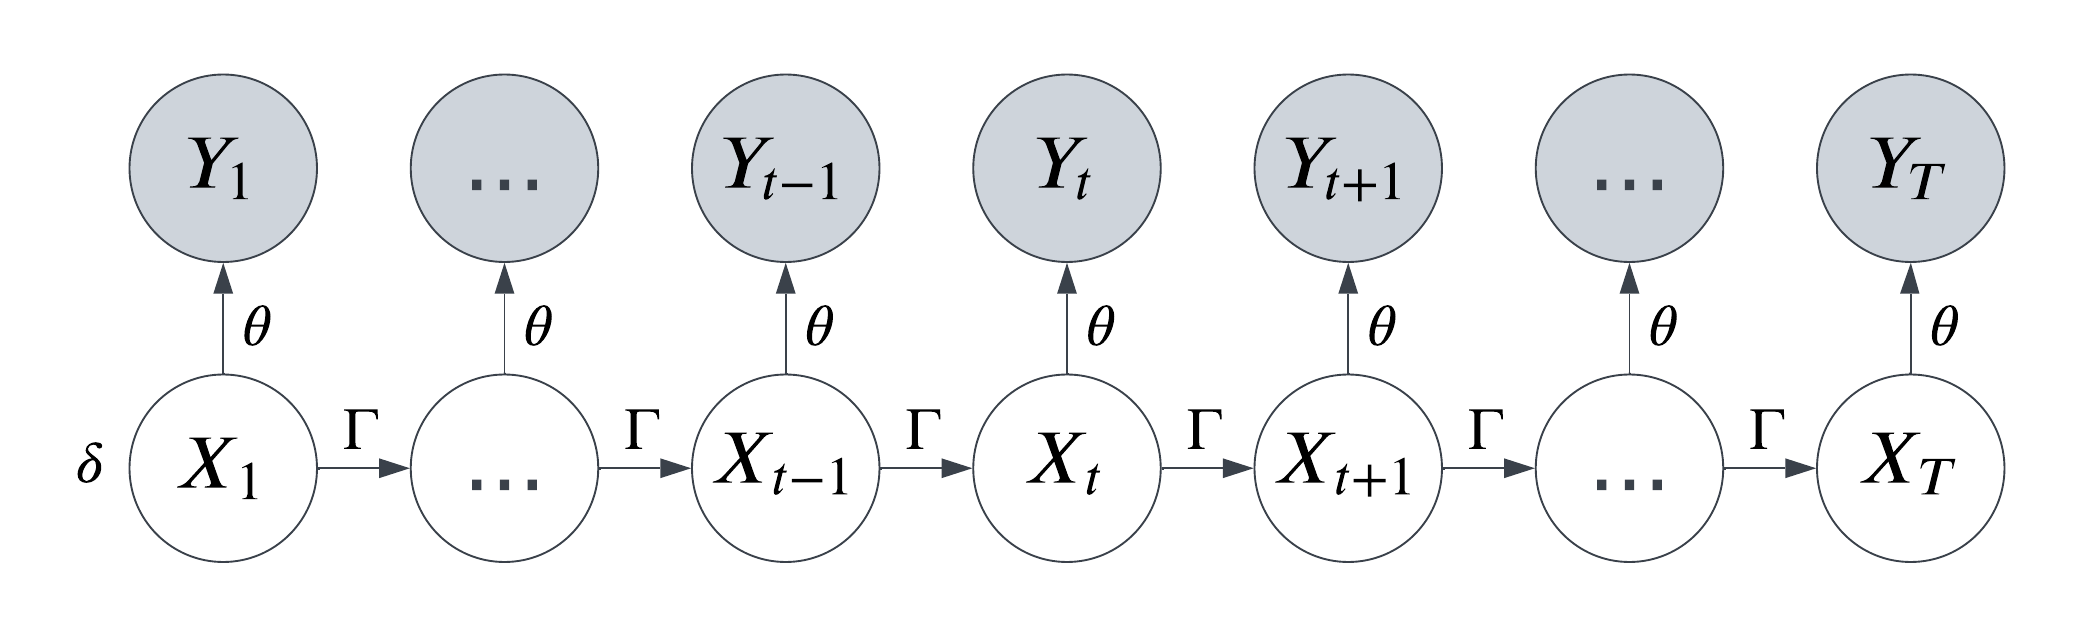
\includegraphics[width=5in]{../plt/HMM.png}
    \caption{Graphical representation of an HMM. $X_t$ corresponds to an unobserved latent state at time $t$ whose distribution is described by a Markov chain. $Y_t$ corresponds to an observation at time $t$, where $Y_t$ given all other observations $\bfY \setminus \{Y_t\}$ and hidden states $\bfX$ depends only on $X_t$.}
    \label{fig:HMM}
\end{figure}

Denote a fixed realization of observations $\bfY$ and latent states $\bfX$ as $\bfy = \{y_t\}_{t=1}^T$ and $\bfx = \{x_t\}_{t=1}^T$. The joint likelihood of an HMM given $\bfy$ and $\bfx$ is
%
\begin{equation}
    p(\bfx,\bfy;\bfphi) = \delta^{(x_1)} f^{(x_1)}(y_1; \theta^{(x_1)}) \prod_{t=2}^T \Gamma^{(x_{t-1},x_t)} f^{(x_t)}(y_t; \theta^{(x_t)}).
    \label{eqn:like}
\end{equation}
%
Alternatively, the marginal likelihood of the observed data $\bfy$ alone is 
%
\begin{equation}
    p(\bfy;\bfphi) = \bfdelta P(y_1;\bftheta) \prod_{t=2}^T \bfGamma P(y_t;\bftheta) \mathbf{1}^\top_N,
    \label{eqn:like_marginal}
\end{equation}
%
where $\mathbf{1}_N$ is an $N$-dimensional row vector of ones and $P(y_t;\bftheta)$ is an $N \times N$ diagonal matrix with entry $(i,i)$ equal to $f^{(i)}(y_t; \theta^{(i)})$. For a more complete introduction to HMMs, see \citet{Zucchini:2016}.
%
\subsection{State Decoding}

One appealing feature of HMMs is that it is simple to determine the distribution of a given hidden state ($X_t$) conditioned on a set of observations $\bfy$. Assuming that the HMM parameters $\bfphi$ are fixed, define the probability density of the observations between times $s$ and $t$ as $p(y_{s:t};\bfphi)$. Likewise, define \textit{forward probabilities} $\alpha^{(i)}_t = p(y_{1:t},X_t = i;\bfphi)$ (for $i = 1,\ldots,N$ and $t = 1,\ldots,T$) and \textit{backward probabilities} $\beta^{(i)}_t = p(y_{(t+1):T} \mid X_t = i;\bfphi)$ (for $i = 1,\ldots,N$ and $t = 1,\ldots,T-1$). By convention, $\beta^{(i)}_T = 1$ for $i = 1,\ldots,N$. We thus define the row vectors $\bfalpha_t = \begin{pmatrix} \alpha_t^{(1)} & \cdots & \alpha_t^{(N)} \end{pmatrix}$ and $\bfbeta_t = \begin{pmatrix} \beta_t^{(1)} & \cdots & \beta_t^{(N)} \end{pmatrix}$ . Both $\bfalpha_t$ and $\bfbeta_t$ can be calculated using the following recursions:

\begin{gather}
    \bfalpha_1 = \bfdelta ~ P(y_1;\bftheta), \qquad 
    %
    \bfalpha_t = \bfalpha_{t-1} ~ \bfGamma ~ P(y_t;\bftheta), \quad t = 2,\ldots,T, \label{eqn:alpha} \\
    %
    \bfbeta^\top_T = \mathbf{1}_N^\top, \qquad
    %
    \bfbeta^\top_t = \bfGamma ~ P(y_{t+1};\bftheta) ~ \bfbeta^\top_{t+1}, \quad t = 1,\ldots,T-1. \label{eqn:beta}
\end{gather}
%
We define conditional probabilities $\gamma_t^{(i)} = \bbP(X_t = i \mid \bfY = \bfy ~;~ \bfphi)$ and $\xi_t^{(i,j)} = \bbP(X_{t-1} = i, X_t = j \mid \bfY = \bfy ~;~ \bfphi)$. We also define the row vector $\bfgamma_t = \begin{pmatrix} \gamma_t^{(1)} & \cdots & \gamma_t^{(N)} \end{pmatrix}$ and the matrix 

\begin{equation*}
    \bfxi_t = \begin{pmatrix} 
    \xi_t^{(1,1)} & \cdots & \xi_t^{(1,N)} \\
    \vdots & \ddots & \vdots \\
    \xi_t^{(N,1)} & \cdots & \xi_t^{(N,N)} \\
    \end{pmatrix}, \qquad t = 2,\ldots,T. 
\end{equation*}
%
Both $\bfgamma_t$ and $\bfxi_t$ can be calculated from $\bfalpha_{t-1}$, $\bfalpha_t$, $\bfbeta_t$, $\bfGamma$, and $\bftheta$. Let $\text{diag}(\cdot)$ map a row vector to the diagonal matrix with that row vector as its diagonal. Then,

\begin{gather}
    \gamma^{(i)}_t = \frac{\alpha^{(i)}_{t} ~ \beta^{(i)}_{t}}{\bfalpha_{t} ~ \bfbeta_t^\top}, \qquad \bfgamma_t = \frac{\bfalpha_t ~ \text{diag}(\bfbeta_t)}{\bfalpha_t ~ \bfbeta_t^\top} \label{eqn:gamma}, \\
    %
    \xi_{t}^{(i,j)} = \frac{\alpha_{t-1}^{(i)} ~ \Gamma^{(i,j)} ~ f^{(j)}(y_{t};\theta^{(j)}) ~ \beta_{t}^{(j)}}{\bfalpha_{t-1} ~ \bfGamma ~ P(y_{t};\bftheta) ~ \bfbeta_{t}^\top}, \qquad \bfxi_t = \frac{\text{diag}(\bfalpha_{t-1}) ~ \bfGamma ~ P(y_t;\bftheta) ~ \text{diag}(\bfbeta_t)}{\bfalpha_{t-1} ~ \bfGamma ~ P(y_{t};\bftheta) ~ \bfbeta_{t}^\top} \label{eqn:xi}.
\end{gather}
%
For shorthand, we define the sets $\{\bfalpha, \bfbeta, \bfgamma, \bfxi\} = \{\bfalpha_t, \bfbeta_t, \bfgamma_t, \bfxi_t\}_{t=1}^T$ to summarize the conditional probabilities for all $t$. In future sections, when $\bfphi$ is not fixed (e.g. during the parameter estimation procedures), we add an argument to the conditional probabilities and write $\{\bfalpha(\bfphi), \bfbeta(\bfphi), \bfgamma(\bfphi), \bfxi(\bfphi)\} = \{\bfalpha_t(\bfphi), \bfbeta_t(\bfphi), \bfgamma_t(\bfphi), \bfxi_t(\bfphi)\}_{t=1}^T$ to highlight the dependence on $\bfphi$. 

\subsection{The Baum-Welch Algorithm}

The Baum-Welch algorithm is an iterative algorithm used to estimate the parameters of an HMM. It predates the more general expectation-maximization (EM) algorithm \citep{Dempster:1977}, but the two are equivalent when applied to HMMs. At iteration $k$ of the EM algorithm, denote the current parameter estimates as $\bfphi_{k}$. One iteration of the EM algorithm consists of an expectation (or E) step, followed by a maximization (or M) step. For the E step, the function value $Q(\bfphi \mid \bfphi_{k})$ is defined as the expected value of the joint log-likelihood $\log p(\bfX,\bfy; \bfphi)$ taken with respect to $\bfX$, where $\bfX$ has conditional probability mass function $p(\bfX \mid \bfY = \bfy ; \bfphi_{k})$. For the M step, the next parameter estimate $\bfphi_{k+1}$ is found by maximizing $Q(\bfphi \mid \bfphi_{k})$ with respect to $\bfphi$:

\begin{gather}
    Q(\bfphi \mid \bfphi_{k}) = \bbE_{\bfphi_{k}}\left[\log p(\bfX,\bfy;\bfphi) \mid \bfY = \bfy \right] \label{eqn:Q}, \\
    %
    %Q^*(\bfphi_{k}) = \max_{\bfphi}Q(\bfphi \mid \bfphi_{k})\\
    %
    \bfphi_{k+1} = \argmax_{\bfphi} Q(\bfphi \mid \bfphi_{k}). \label{eqn:BW_update}
\end{gather}
%
For notational convenience, we occasionally denote the set of conditional probabilities $\{\bfalpha_t(\bfphi_k), \bfbeta_t(\bfphi_k), \bfgamma_t(\bfphi_k), \bfxi_t(\bfphi_k)\}$ as $\{\bfalpha_{k,t},\bfbeta_{k,t},\bfgamma_{k,t},\bfxi_{k,t}\}$. Substituting Equation (\ref{eqn:like}) into Equation (\ref{eqn:Q}) and performing some algebra yields a closed form expression for $Q$: 
%
\begin{equation}
    Q(\bfphi \mid \bfphi_{k}) = \sum_{i=1}^N \gamma^{(i)}_{k,1} \log \delta^{(i)}(\bfnu) + \sum_{t = 1}^T \sum_{i=1}^N \gamma^{(i)}_{k,t} \log f^{(i)}(y_t;\theta^{(i)}) + \sum_{t=2}^{T} \sum_{i=1}^N \sum_{j=1}^N \xi^{(i,j)}_{k,t} \log \Gamma^{(i,j)}(\bfeta).
    \label{eqn:Q_sum}
\end{equation}
%
The conditional probabilities $\gamma_{k,t}^{(i)}$ and $\xi_{k,t}^{(i,j)}$ thus act as weights for $\log \delta^{(i)}(\bfnu)$, $\log f^{(i)}(y_t;\theta^{(i)})$, and $\log \Gamma^{(i,j)}(\bfeta)$ for $i,j = 1,\ldots,N$. We thus refer to $\bfgamma$ and $\bfxi$ as weights in future sections. Detailed pseudocode for the E and the M step are given in Algorithms \ref{alg:E} and \ref{alg:EM} below.
%
\begin{algorithm}
\caption{\texttt{E-step}($\bfphi$)}\label{alg:E}
\begin{algorithmic}[1]
\Require Parameter value $\bfphi = \{\bftheta,\bfeta,\bfnu\}$.
%
\State $\bfdelta = \bfdelta(\bfnu), \quad \bfGamma = \bfGamma(\bfeta)$
\State $\bfalpha_1 = \bfdelta ~ P(y_1;\bftheta)$
\State $\bfbeta^\top_T = \mathbf{1}_N^\top$
\For{$t = 2,\ldots,T$}
    \State $$\bfalpha_t = \bfalpha_{t-1} ~ \bfGamma ~ P(y_t;\bftheta), \qquad \bfbeta^\top_{T-t+1} = \bfGamma ~ P(y_{T-t+2};\bftheta) ~ \bfbeta^\top_{T-t+2}$$
\EndFor
%
\State $\bfgamma_1 = \frac{\bfalpha_1 ~ \text{diag}(\bfbeta_1)}{\bfalpha_1 ~ \bfbeta_1^\top}$
%
\For{$t = 2,\ldots,T$}
    \State $$\bfgamma_t = \frac{\bfalpha_t ~ \text{diag}(\bfbeta_t)}{\bfalpha_t ~ \bfbeta_t^\top}, \qquad \bfxi_t = \frac{\text{diag}(\bfalpha_{t-1}) ~ \bfGamma ~ P(y_t;\bftheta) ~ \text{diag}(\bfbeta_t)}{\bfalpha_{t-1} ~ \bfGamma ~ P(y_{t};\bftheta) ~ \bfbeta_{t}^\top}$$
\EndFor
%
\State \Return $\{\bfalpha_t,\bfbeta_t,\bfgamma_t,\bfxi_t\}_{t=1}^T$
\end{algorithmic}
\end{algorithm}
%
%
%
\begin{algorithm}
\caption{\texttt{Baum-Welch}$(\bfphi_0,K)$}\label{alg:EM}
\begin{algorithmic}[1]
\Require Initial parameter values $\bfphi_0$, number of iterations $K$
\For{$k = 0,\ldots,K-1$}
    \State $\{\bfalpha_{k,t},\bfbeta_{k,t},\bfgamma_{k,t},\bfxi_{k,t}\}_{t=1}^T = \texttt{E-step}(\bfphi_{k})$ \Comment{E step} 
    \State \Comment{M step} \small $$\bfphi_{k+1} = \argmax_{\{\bftheta,\bfeta,\bfnu\}} \sum_{i=1}^N \gamma^{(i)}_{k,1} \log \delta^{(i)}(\bfnu) + \sum_{t = 1}^T \sum_{i=1}^N \gamma^{(i)}_{k,t} \log f^{(i)}(y_t;\theta^{(i)}) + \sum_{t=2}^{T} \sum_{i=1}^N \sum_{j=1}^N \xi_{k,t}^{(i,j)} \log \Gamma^{(i,j)}(\bfeta)$$ \normalsize
\EndFor
\State \Return $\bfphi_K$
\end{algorithmic}
\end{algorithm}
%
In some simple scenarios, the maximization problem in Equation (\ref{eqn:BW_update}) above has a closed-form solution. However, this maximization problem is not always straightforward and often requires numerical maximization techniques. We thus review different methods for numerical maximization via stochastic optimization.

\subsection{Stochastic Optimization}
\label{subsec:stoch_optim}

Stochastic optimization involves a class of optimization methods that use random variables to maximize or minimize an objective function. We focus on optimization methods to minimize objective functions that can be written as a sum of many terms \citep{Robbins:1951}, namely to solve
%
\begin{equation}
    \bfphi^* = \argmin_{\bfphi} F(\bfphi), \quad \text{where} \quad F(\bfphi) = \frac{1}{T}\sum_{t = 1}^T F_t(\bfphi).
    \label{eqn:stoch_opt}
\end{equation}
%

We denote the parameter values at step $m$ of an optimization scheme as $\bfphi^{(m)} = \{\bftheta^{(m)},\bfeta^{(m)},\bfnu^{(m)}\}$ to distinguish between the parameter values $\bfphi_k$ at iteration $k$ of the Baum-Welch algorithm. The bold parameters $\bftheta^{(m)}$, $\bfeta^{(m)}$, and $\bfnu^{(m)}$ correspond to optimization step $m$ and are not to be confused with $\theta^{(i)}$, $\eta^{(i,j)}$, and $\nu^{(i)}$ which correspond to hidden states $i$ and $j$ of the HMM. Standard gradient descent at a given step $m$ with step size $\lambda$ updates the parameter value $\bfphi^{(m)}$ by moving in the direction of the negative gradient of $F$. Formally, the update step is $\bfphi^{(m+1)} = \bfphi^{(m)} - \lambda \nabla F(\bfphi^{(m)})$, or $\bfphi^{(m+1)} = \bfphi^{(m)} - (\lambda/T) \sum_{t=1}^T \nabla F_t(\bfphi^{(m)})$ for our problem. The step size $\lambda$ is user-defined. It should be large enough so $\bfphi^{(m+1)}$ moves quickly towards a minimum of $F$, but not so large that $\bfphi^{(m+1)}$ ``overshoots" the minimum. This update requires evaluating a gradient for all $t = 1,\ldots,T$, which can be prohibitively expensive if $T$ is large.

In contrast, stochastic gradient descent (SGD) updates $\bfphi$ using $\bfphi^{(m+1)} = \bfphi^{(m)} - \lambda_m \nabla F_{t_m}(\bfphi^{(m)}),$ where $t_m \in \{1,\ldots,T\}$ is selected uniformly at random at step $m$ of the algorithm \citep{Robbins:1951}. Stochastic gradient descent reduces the amount of time between updates by using an unbiased estimate of the gradient to update $\bfphi^{(m)}$. However, the gradient estimates can have very high variance, so stochastic gradient descent requires that the step size $\lambda_m$ is smaller than that of full gradient descent. The step size must also decay to zero as $m \to \infty$ to ensure convergence. Further, SGD has slower convergence rates than full gradient descent \citep{Schmidt:2017}.

Variance-reduced stochastic optimization techniques such as stochastic average gradient (SAG) \citep{Schmidt:2017}, stochastic variance reduced gradient (SVRG) \citep{Johnson:2013}, and stochastic average gradient accelerated (SAGA) \citep{Defazio:2014} enjoy the speed of stochastic gradient descent as well as the convergence rates of full gradient descent. These algorithms involve storing gradient approximations at each gradient step $m$, $\widehat \nabla F_{t}^{(m)}$ for $t = 1,\ldots,T$, whose average approximates the full gradient $\nabla F(\bfphi^{(m)})$. The gradient approximations are updated at various stages in the optimization algorithm and are used to reduce the variance of the full gradient estimate. For example, SVRG and SAGA update $\bfphi^{(m)}$ via $\bfphi^{(m+1)} = \bfphi^{(m)} - \lambda_m \left[\nabla F_{t_m}(\bfphi^{(m)}) - \widehat \nabla F_{t_m}^{(m)} + \widehat \nabla F^{(m)} \right],$ where $t_m \in \{1,\ldots,T\}$ is chosen uniformly at random and $\widehat \nabla F^{(m)} = (1/T) \sum_{t=1}^T \widehat \nabla F_{t}^{(m)}$.
%
Like SGD, this stochastic update has the same expectation as that of standard gradient descent, but it empirically exhibits lower variance than SGD and it is guaranteed to converge without decaying the step size $\lambda_m$ (under certain regularity conditions). After updating the parameters at step $m$, SAGA updates the gradient approximation $\widehat \nabla F_{t_m}^{(m+1)}$ and recalculates the resulting gradient average $\widehat \nabla F^{(m+1)}$.
%
Algorithm \ref{alg:VRSO} outlines SVRG and SAGA in pseudocode, and we denote it as \textit{variance-reduced stochastic optimization}, or $\texttt{VRSO}$. 

\begin{algorithm}
\caption{\texttt{VRSO}$(F,\bfphi^{(0)},\lambda,A,M)$}\label{alg:VRSO}
\begin{algorithmic}[1]
\Require Loss function $F = \frac{1}{T}\sum_{t=1}^T F_t$, initial value $\bfphi^{(0)}$, step size $\lambda$, algorithm $A \in \{\text{SVRG, SAGA}\}$, and number of iterations $M$.
%
\vspace{5pt}
\For{$t = 1,\ldots,T$} \Comment{initialize gradients}
\State $\widehat \nabla F_{t}^{(0)} = \nabla F_t (\bfphi^{(0)})$
\EndFor
\State $\widehat \nabla F^{(0)} = (1/T) \sum_{t=1}^T \widehat \nabla F_{t}^{(0)}$
%
\For{$m = 0,\ldots,M-1$}
    %
    \State Pick $t_m \in \{1,\ldots,T\}$ uniformly at random.
    %
    \State \Comment{update parameters}
    \begin{gather}
        \bfphi^{(m+1)} = \bfphi^{(m)} - \lambda \left[\nabla F_{t_m}(\bfphi^{(m)}) - \widehat \nabla F_{t_m}^{(m)} + \widehat \nabla F^{(m)} \right]
        \label{eqn:SAGA_update0}
    \end{gather}
    %
    \State $\widehat \nabla F_{t}^{(m+1)} = \widehat \nabla F_{t}^{(m)} \enspace$ for $t = 1,\ldots,T$ 
    %
    \Comment{update gradient approximations and average}
    %
    \If{$A$ = SAGA}:
        \begin{gather}
            \widehat \nabla F_{t_m}^{(m+1)} = \nabla F_{t_m}(\bfphi^{(m)}) \\
            \widehat \nabla F^{(m+1)} = \widehat \nabla F^{(m)} + \frac{1}{T} \left(\widehat \nabla F_{t_m}^{(m+1)} - \widehat \nabla F_{t_m}^{(m)}\right)
        \end{gather}
    \EndIf
\EndFor
\State \Return $\bfphi^{(M)}$
\end{algorithmic}
\end{algorithm}

SAGA involves running Algorithm \ref{alg:VRSO} until convergence. However, the gradient approximations $\widehat \nabla F_{t}^{(m)}$ are never updated when using SVRG within Algorithm \ref{alg:VRSO}. As such, SVRG requires repeatedly running Algorithm \ref{alg:VRSO} with $M$ scaling approximately with $T$ so the set of gradient approximations remains up-to-date.